% =====================================================================
\section{Dynamics: the attracting fixed point}\label{sec:dynamics}
% =====================================================================

Because $0 < \Tah'(y) \le 1$ everywhere with equality only at the
origin (Proposition~\ref{prop:lipschitz}), the Tahawus function is a
weak contraction of $\R$ into $(0,\infty)$, and its iteration theory
is as clean as one could hope: there is a single fixed point, it
attracts everything, and every orbit approaches it monotonically.

\begin{theorem}[fixed point]\label{thm:fixedpoint}
\begin{enumerate}[label=\textup{(\roman*)}, leftmargin=2.4em]
\item $\Tah$ has a unique fixed point
\[
    \delta \;=\; 2.2288331032781189706187615546\ldots,
    \qquad
    \delta^{\,\delta} \;=\; \delta^{2} + 1 ,
\]
which is the unique positive root of $x^{x} = x^{2}+1$ and lies in
$(2,3)$.
\item $\delta$ is transcendental.
\item Every orbit $y_{n+1} = \Tah(y_{n})$ converges to $\delta$:
strictly increasing if $y_{0} < \delta$, strictly decreasing if
$y_{0} > \delta$ (after one step from any $y_{0} \le 0$).
\item The fixed point is attracting, with
$\Tah'(\delta) = 0.2615\ldots < 1$.
\end{enumerate}
\end{theorem}

\begin{proof}
(i) For $y > 0$, $\Tah(y) = y \iff y^{y} - 1 = y^{2} \iff h(y) := y^{y}
- y^{2} - 1 = 0$; and no $y \le 0$ is fixed since $\Tah(y) > 0 \ge y$
with $\Tah(0) = 1$. Now $h < 0$ on $(0,2]$: for $0 < x < 1$,
$x^{x} < 1 < 1 + x^{2}$; for $1 \le x \le 2$, $x^{x-2} \le 1$ gives
$x^{x} \le x^{2} < x^{2}+1$. On $(2,\infty)$ write
$h(x) = x^{2}\bigl(x^{x-2} - 1 - x^{-2}\bigr)$, whose sign is the sign
of
\[
    K(x) := (x-2)\ln x - \ln\bigl(1 + x^{-2}\bigr), \qquad
    K'(x) = \ln x + \frac{x-2}{x} + \frac{2}{x(x^{2}+1)} \;>\; 0 :
\]
each term is positive for $x > 2$. Since $K(2) = -\ln\tfrac54 < 0 <
\ln 3 - \ln\tfrac{10}{9} = K(3)$, $h$ has exactly one zero
$\delta \in (2,3)$.

(iii) $\Tah(y) > y \iff h(y) < 0$ (apply the increasing $f$ to both
sides: $\Tah(y) > y \iff y = f(\Tah(y)) > f(y)$, and
$f(y) - y = h(y)/y$). So $\Tah(y) > y$ on $(0,\delta)$ and
$\Tah(y) < y$ on $(\delta,\infty)$. As $\Tah$ is increasing with
$\Tah(\delta) = \delta$, it maps $(0,\delta)$ into $(0,\delta)$ and
$(\delta,\infty)$ into $(\delta,\infty)$; monotone bounded sequences
converge, and continuity forces the limit to be a fixed point. For
$y_{0} \le 0$, $y_{1} = \Tah(y_{0}) \in (0,1] \subset (0,\delta)$.

(ii) If $\delta$ were an algebraic irrational, Gelfond--Schneider
would make $\delta^{\delta}$ transcendental, contradicting
$\delta^{\delta} = \delta^{2} + 1$ algebraic. If $\delta = p/q$ (lowest
terms, $p > q$ since $\delta > 2$), then raising
$(p/q)^{p/q} = (p^{2}+q^{2})/q^{2}$ to the $q$-th power gives
$p^{p}\, q^{\,2q-p} = (p^{2}+q^{2})^{q}$. But
$\gcd\bigl(p,\, p^{2}+q^{2}\bigr) = \gcd(p, q^{2}) = 1$, so any prime
$\ell \mid p$ has $v_\ell(\text{LHS}) = p\,v_\ell(p) > 0$ (as
$\ell \nmid q$) while $v_\ell(\text{RHS}) = 0$: impossible. Hence
$p = 1$, contradicting $p > q \ge 1$. So $\delta$ is transcendental.

(iv) $\Tah'(\delta) = \delta^{2}/f'(\delta)$ with
$f'(\delta) = \delta^{\delta-1}\bigl(\ln\delta + 1 -
\tfrac1\delta\bigr) + \delta^{-2} = 9.382\ldots$, giving
$\Tah'(\delta) = 0.2615435596\ldots$; it is $< 1$ by
Proposition~\ref{prop:lipschitz}.
\end{proof}

\begin{figure}[t]
    \centering
    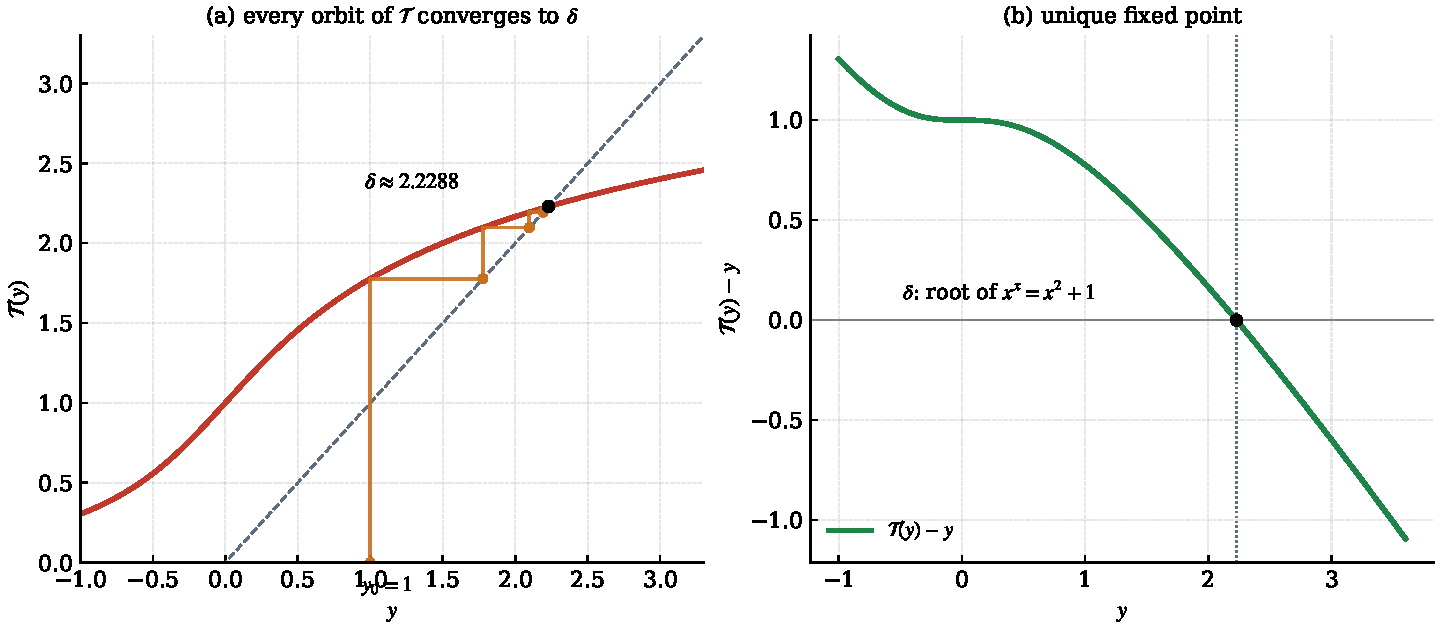
\includegraphics[width=0.98\textwidth]{figures/fig5_orbit.pdf}
    \caption{(a) Staircase diagram of the orbit of $\Tah$ started at
    $y_{0} = 1$ (orange): the orbit climbs monotonically to the
    attracting fixed point $\delta \approx 2.2288$ (black dot), where
    the graph of $\Tah$ (red) crosses the diagonal (dashed).
    (b) The displacement $\Tah(y) - y$: positive exactly on
    $(0, \delta)$, vanishing at the unique fixed point, root of
    $x^{x} = x^{2}+1$.}
    \label{fig:orbit}
\end{figure}

The orbit of $1$ is a good advertisement for the speed of the
attraction, and for how quickly the iterates forget that they started
at the Tahawus constant:
\[
\begin{aligned}
    &1,\; 1.7767750401,\; 2.0971558587,\; 2.1933551737,\;
    2.2194806484,\\
    &2.2263819619,\; 2.2281916756,\; 2.2286653182,\;
    2.2287892186,\; 2.2288216254,\;\ldots\;\to\;\delta,
\end{aligned}
\]
each step multiplying the error by roughly $\Tah'(\delta) = 0.2615$.
An orbit started at $y_{0} = -5$ reaches $0.00622$, then $1.00622$,
then follows the same staircase: one step suffices to enter
$(0,\delta)$, as promised. Newton's method on
$g(x) = x^{x} - x^{2} - 1$, started at $2$, exhibits its usual
quadratic convergence:
$2.36067$, $2.25177$, $2.22964$, $2.22883$, $2.228833103278118971$.
We remark that $\delta$ is the $n = 2$ member of the family of
\emph{super-golden} constants $\{$roots of $x^{x} = x^{n} + 1\}$,
whose first member ($n = 1$) is $\alpha$ itself; see Open
Problem~\ref{op:family}.

\subsection{The nested composition of the blog post, made convergent}
\label{subsec:W-iteration}

The infinite composition \eqref{eq:W-nest} is not a closed form, but
it \emph{is} a numerical algorithm: read from the outside in, it is
the fixed-point iteration
\begin{equation}\label{eq:W-iteration}
    x_{n+1} \;=\; \ssqrt(x_{n} + 1) \;=\; \ee^{W(\ln(x_{n}+1))},
    \qquad x_{0} \;=\; \ssqrt(2) = \ee^{W(\ln 2)},
\end{equation}
where the starting value is the first approximant obtained by ignoring
the ``$+1$'' (this is exactly the nesting displayed in the original
post). The remarkable fact is that this iteration is a
\emph{contraction with a closed-form rate}, in sharp contrast with the
power-tower iteration of the next section.

\begin{proposition}[the $W$-iteration converges geometrically]
\label{prop:W-iteration}
Let $g(x) := \ssqrt(x+1) = \ee^{W(\ln(x+1))}$ on $[0,\infty)$. Then
$g$ is increasing, $g(x) > x$ on $[0, \alpha)$, $g(x) < x$ on
$(\alpha, \infty)$, and every orbit of \eqref{eq:W-iteration}
converges monotonically to $\alpha$. Moreover $g$ is differentiable at
$\alpha$ with
\begin{equation}\label{eq:W-rate}
    g'(\alpha) \;=\; \frac{1}{(1 + \alpha)\bigl(1 + \ln \alpha\bigr)}
    \;=\; 0.2286830163\ldots \;<\; 1 ,
\end{equation}
so the convergence is geometric with ratio \eqref{eq:W-rate}.
\end{proposition}

\begin{proof}
Monotonicity of $g$ is that of $x \mapsto x + 1$, $\ln$, $W$ and
$\exp$. For $x \in [0,1)$ we have $g(x) \ge \ssqrt(1) = 1 > x$. For
$x \ge 1$ (where $t \mapsto t^{t}$ is increasing), $g(x) > x \iff
x^{x} < x + 1 \iff x < \alpha$; this uses the (known) fact that
$x^{x} - x - 1$ is strictly increasing on $[1,\infty)$, with root
$\alpha$. Hence $g$ maps $[0, \alpha]$ into $[1, \alpha]$ and
$(\alpha, \infty)$ into $(\alpha, \infty)$ with $g(x) < x$ there, and
monotone convergence proceeds exactly as in
Theorem~\ref{thm:fixedpoint}(iii), the only fixed point of $g$ in
$[0,\infty)$ being $\alpha$. For the rate:
$g'(x) = g(x)\, W'(\ln(x+1))\,/(x+1)$ with
$W'(z) = W(z)/\bigl(z(1+W(z))\bigr)$; at $x = \alpha$ we have
$g(\alpha) = \alpha$ and $W(\ln(\alpha+1)) = \ln\alpha$, because
$(\ln\alpha)\,\ee^{\ln\alpha} = \alpha\ln\alpha =
\ln(\alpha^{\alpha}) = \ln(\alpha+1)$. Substituting $z = \ln(\alpha+1)
= \alpha \ln \alpha$,
\[
    g'(\alpha)
    \;=\; \alpha \cdot \frac{\ln\alpha}{\alpha\ln\alpha\,
    (1 + \ln\alpha)} \cdot \frac{1}{\alpha + 1}
    \;=\; \frac{1}{(1+\alpha)(1+\ln\alpha)} .
    \qedhere
\]
\end{proof}

The first iterates of \eqref{eq:W-iteration} are
\[
    1.55961,\; 1.7245718243,\; 1.7646972820,\; 1.7740056666,\;
    1.7761413436,\; \ldots,\;
    1.7767750401 \;=\; \alpha ,
\]
reaching $\alpha$ to nine significant digits in eight steps; the
observed error ratios $0.23136$, $0.22930$, $0.22882$, $0.22872$,
$0.22869$, $0.228685$,~\ldots{} march to the closed form
\eqref{eq:W-rate} exactly.
This is the honest content of the blog post's nested expression: not
a closed form, but a rapidly convergent evaluation scheme. The same
scheme works verbatim for general $b$, iterating
$x \mapsto \ee^{W(\ln(bx+1))}$.

% =====================================================================
\section{The infinite power tower, corrected}\label{sec:tower}
% =====================================================================

The original post closes with a flourish: since
\begin{equation}\label{eq:blog-tower}
    \alpha^{\alpha} \;=\; \alpha + 1,
    \qquad\text{i.e.}\qquad
    \alpha^{\alpha} - 1 \;=\; \alpha ,
\end{equation}
the constant $\alpha$ can be substituted into itself forever,
\[
    \alpha \;=\; \alpha^{\alpha} - 1 \;=\;
    \alpha^{\alpha^{\alpha} - 1} - 1 \;=\;
    \alpha^{\alpha^{\alpha^{\alpha} - 1} - 1} - 1 \;=\; \cdots,
\]
an identity of infinite nested exponentials with a ``$-1$'' attached
at every level. As an \emph{algebraic} identity the chain is
unimpeachable: the sequence $x_{n+1} = \alpha^{x_{n}} - 1$ started at
$x_{0} = \alpha$ is exactly constant. As a statement about a
\emph{limit}, however---the natural reading of an infinite
expression---it is wrong, and the correction is instructive.

\begin{theorem}[the decremented tower]\label{thm:tower}
Let $1 < a < \ee$, let $g_{a}(x) := a^{x} - 1$, and let $x_{+}(a) >
0$ denote the unique positive solution of $a^{x} = x + 1$ (it exists
and is unique). Then:
\begin{enumerate}[label=\textup{(\roman*)}, leftmargin=2.4em]
\item $g_{a}$ has exactly two nonnegative fixed points, $0$ and
$x_{+}(a)$.
\item The fixed point $0$ is attracting, with multiplier
$g_{a}'(0) = \ln a < 1$; the fixed point $x_{+}(a)$ is
\emph{repelling}: its multiplier satisfies
\begin{equation}\label{eq:repelling}
    g_{a}'\bigl(x_{+}(a)\bigr) \;=\; \bigl(x_{+}(a) + 1\bigr)\ln a
    \;=\; \frac{x_{+}(a) + 1}{x_{+}(a)}\,\ln\!\bigl(x_{+}(a)+1\bigr)
    \;>\; 1 ,
\end{equation}
by the inequality $\ln(1+u) > u/(1+u)$ for $u > 0$.
\item Every orbit started in $(-1, x_{+}(a))$ converges
\emph{monotonically} to $0$; every orbit started above
$x_{+}(a)$ diverges monotonically to $+\infty$; the orbit started
exactly at $x_{+}(a)$ is stationary.
\end{enumerate}
For the Tahawus constant, $a = \alpha \in (1, \ee)$ and
$x_{+}(\alpha) = \alpha$ (this is \eqref{eq:blog-tower}), so the
decremented tower built on $\alpha$ converges to $0$ from every
starting point except $\alpha$ itself, where it is stationary, and
above which it diverges.
\end{theorem}

\begin{proof}
Put $h_{a}(x) := a^{x} - x - 1 = g_{a}(x) - x$. Then
$h_{a}(0) = 0$, $h_{a}'' = (\ln a)^{2} a^{x} > 0$, and
$h_{a}'(x) = \ln(a)\,a^{x} - 1$ is strictly increasing with
$h_{a}'(0) = \ln a - 1 < 0$ and $h_{a}' \to \infty$. So $h_a$
decreases from $h_{a}(0) = 0$ on $[0, x^{*}]$ (where $x^{*}$ is the
zero of $h_{a}'$), hence is negative on $(0, x^{*}]$, and then
increases to $+\infty$, crossing zero exactly once more at
$x_{+}(a) > x^{*}$. On $(-1, 0)$: $h_{a}$ is decreasing there (as
$(-1,0) \subset (-\infty, x^{*})$) with $h_{a}(0) = 0$, so
$h_{a} > 0$ on $(-1, 0)$: no negative fixed points; and points
$x \le -1$ are mapped into $(-1, 0)$ in one step since
$g_{a}(x) \in (-1, a^{-1} - 1] \subset (-1, 0)$. The sign of
$g_{a}(x) - x = h_{a}(x)$ is thus $+$, $-$, $+$ on the intervals
$(-1,0)$, $(0, x_{+})$, $(x_{+}, \infty)$, and $g_{a}$ maps each of
the first two intervals into itself, giving monotone convergence to
the unique fixed point of each interval, namely $0$; on the third
interval the orbit increases without fixed points above, so it
diverges. The multipliers are $g_{a}'(x) = \ln(a)\,a^{x}$: at $0$
this is $\ln a < 1$; at $x_{+}$, using $a^{x_{+}} = x_{+}+1$,
$g_{a}'(x_{+}) = (x_{+}+1)\ln a = \frac{x_{+}+1}{x_{+}}
\ln(x_{+}+1) > 1$ by $\ln(1+u) > \frac{u}{1+u}$.
\end{proof}

For $a = \alpha$ the multipliers come out as
\[
    g_{\alpha}'(0) \;=\; \ln\alpha \;=\; 0.5747999458\ldots,
    \qquad
    g_{\alpha}'(\alpha) \;=\; (1+\alpha)\ln\alpha \;=\;
    1.5960901426\ldots \;>\; 1 ,
\]
and the orbit started at $x_{0} = \tfrac12$ tells the whole story:
\[
    0.3330,\; 0.2109,\; 0.1289,\; 0.0769,\; 0.0452,\; 0.0263,\;
    0.0152,\; 0.0088,\; 0.0051,\; 0.0029,\; \ldots \;\to\; 0 ,
\]
with successive ratios $0.633, 0.611, 0.597, \ldots$ settling toward
the predicted $\ln\alpha = 0.5748$; by step $29$ the iterate is
$4.5 \times 10^{-8}$. So the corrected reading of the post's
identity is:

\begin{quote}
\emph{The decremented tower of base $\alpha$ converges---but to
$0$, not to $\alpha$. The value $\alpha$ is reachable only by the
exactly stationary (and repelling) orbit, which is an algebraic
identity, not a limit process.}
\end{quote}

Two footnotes complete the picture. First, the plain (undecremented)
tower $\alpha^{\alpha^{\alpha^{\cdots}}}$ does not converge at all:
Euler's criterion \cite{knoebel} requires the base to lie in
$[\ee^{-\ee}, \ee^{1/\ee}]$, and $\alpha = 1.7767\ldots$ exceeds
$\ee^{1/\ee} = 1.4446678\ldots$. The decrements do tame the
divergence, but the tamed limit is $0$. Second, the contrast between
Sections~\ref{subsec:W-iteration} and this one is stark and
practical: \emph{the same fixed point} $\alpha$ is repelling for the
map $x \mapsto \alpha^{x} - 1$ (multiplier $1.596$) and attracting
for the map $x \mapsto \ee^{W(\ln(x+1))}$ (multiplier $0.229$), which
are algebraically the same equation. The nest of the blog post should
always be evaluated through $W$, never through the power.

\begin{remark}[general bases]
Theorem~\ref{thm:tower} is stated for the Tahawus constant but proved
for every base $1 < a < \ee$: the pair of fixed points
$\{0, x_{+}(a)\}$ always exists, $0$ always attracts, and
$x_{+}(a)$ always repels, with \eqref{eq:repelling} holding for every
$a$. For $a \ge \ee$ even the fixed point $0$ loses stability
(multiplier $\ln a \ge 1$) and no positive fixed point exists. The
Tahawus constant is simply the special base $a$ for which the
repelling fixed point happens to \emph{coincide with the base
itself}---the self-referential charm that motivated the original
post's identity \eqref{eq:blog-tower}.
\end{remark}
